%!TEX root = ../MasterThesis.tex

\section{The Semantic Web}
\label{sec:semantic_web}

\subsection{Vision}
\label{sec:semantic_vision}

MKP Chapter 1: \\
integrate distributed data from various publishers on the Web into smart applications \\
the Semantic Web delivers the infrastructure for this vision in form of various standard
specifications (RDF, RDFS, OWL, SPARQL, ...) \\
the fundamentals of the World-Wide Web are also supported by the Semantic Web, especially: \\
- AAA-Slogan: Anyone can say Anything about Any topic \\
- Open World Assumption: we must always assume that there exist new information unknown to us yet,
that can give additional insights \\
- Non-unique Naming Assumption: different URIs might refer to the same entity or object \\
\\
as of this any one can extend on existing data entities and contribute her own knowledge / opinions as
well as combine existing information in new ways -> data wilderness, no common data schema, more of an
organic, living system \\
it heavily depends on the ``network effect'' and will / might explode with rising number of users / applications \\
as there will be disagreements on all sorts of topics there is no single ontology for the whole Web,
but rather multiple ontologies tat can be integrated and utilised \\
\\

MIT Chapter 1: \\
make information on the Web accessible to machines \\
- allows integration of information across web sites \\
- is also known as the ``Web of Data'' \\
\\
design principles: \\
1. make structured and semi-structured data available in standardized formats \\
2. make individual data elements and their relationships accessible on the Web \\
3. describe the intended semantics of the data in a machine readable format \\
\\
HTML is just for human consumption and a lot of the structures and semantics of the
underlying databases is lost in the transformation process \\
- use labeled graphs as data model for objects and their relationships (objects == nodes,
edges == relationships between them) \\
- formalize the syntax of the graph in RDF (Resource Description Framework) \\
- use URIs to identify individual data items and relations \\
- use ontologies to represent semantics of the data items (either lightweight RDF schema definitions
or Web Ontology Language are used for that) \\
\\
RDFS and OWL are meta-description languages allowing to define new domain-specific knowledge representations \\
they rely on the basic principles of the Web: supporting distributed, decentralized architectures \\
\\
some new initiatives for standardizing semantics: schema.org and linkeddata.org \\
initially it was tried to solve the integration issues with XML, but as it is syntactically more machine-
readable it lacks the semantic of the data \\
- as of this RDF is the basic language of the Semantic Web and describes meta-data as well as content \\
\\
an ontology formally describe a domain based on terms and their relationships (terms == classes of objects) \\
hierarchies are supported (even multiple inheritance between objects) \\
ontologies also include: \\
- properties \\
- value restrictions \\
- disjointness statements \\
- specifications of logical relationships \\
goal is to provide a shared understanding of a domain \\
can help with the necessity to overcome differences in terminology \\
a mapping for different wordings in an ontology or between ontologies is possible \\
they can also be useful for generalization or specialization of Web search results \\
\\
ontologies help with reasoning of objects, they can uncover unexpected relationships and
inconsistencies as well as - by utilizing intelligent web agents - make decisions and select course of actions
(e.g. ``if-then-conclusions'' aka Horn logic) \\
agents can also be used for ``validation of proof'' of statements of another agent or machine \\
\\
Semantic Web is a layered approach \ldots

\begin{figure}[H]
	\centering
		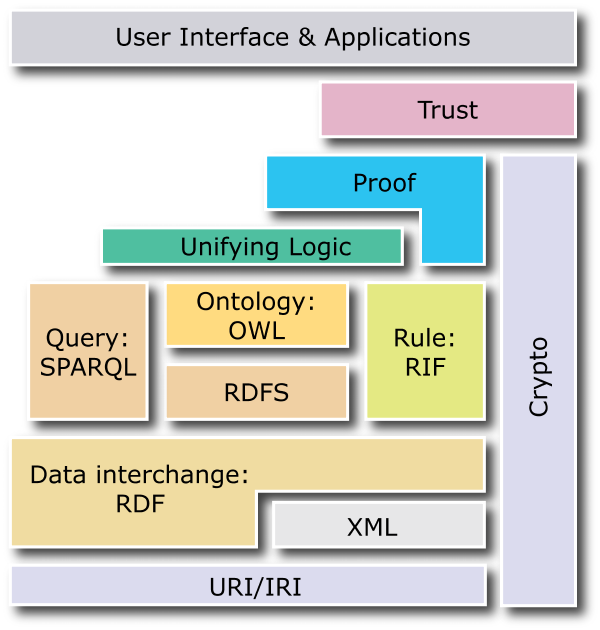
\includegraphics[height=2.5in]{images/semantic_web_layers.png}
	\caption{The Semantic Web Model \citep{W3C2013}}
\label{fig:images_semweb_model}
\end{figure}

% section semantic_vision (end)

\subsection{Semantic Modelling}
\label{sec:semantic_models}

MKP Chapter 2: \\
semantic models \\
- help people communicate about a fact or situation in the world \\
- explain and make predictions about the world \\
- mediate among multiple viewpoints and allow to explore commonalities as well as differences \\
\\
1. human communication and modelling: \\
- helps people to coordinate their understanding collaboratively \\
- knowledge will be gathered, organized, tagged and shared \\
- when building models in natural human language they are usually open for interpretation of the meaning (e.g. laws)  \\
- interpretation of the text depends on time and context of use -> informal model \\
- the success of informal models can be measured as degree of people supporting the intended purpose \\
- tagging systems provide an informal organisation to a large body of heterogenous information \\
- in addition: models can have different layers with an increasing degree of formality (e.g. in the sector of regulations
and laws there are regional, national as well as international laws with different degree of formality) \\
- informal models might be fitting their purpose in the context of their creation, but might need additional layers of models
when their usage get beyond that original context to represent the shared meaning \\
\\
2. explanations and predictions: \\
- help individuals to draw their own conclusions based on the information received \\
- especially useful in ``interpretive situations'' -> something is not set in stone \\
- explanation plays a crucial role in the ``understanding'' of a situation; if someone can ``explain'' it,
they usually understood it \\
- in the Semantic Web explanation might help reuse the whole or parts of an existing model \\
- prediction is closely related to explanation; if a model offer an explanation for a certain situation,
it can also be used to make predictions \\
- that resembles the fundamental of the scientific method (falsification) \\
- explanation and prediction require a more formal models than used for human communication (see above) \\
- usually they are build up from objective statements that are used to describe principles and rules (aka formalism) \\
- these models can also be used to make predictions \\
- they allow to evaluate the validity of a model and its applicability to a given situation \\
- in opposite to human communication formalism doesn't need extra layers of explanations \\
- in the Semantic Web there are certain standards (a formalism) for modelling explanations \\
- these techniques can also be used to validate proofs and make predictions (aka inference) \\
\\
3. Mediating Variability: \\
- goes hand in hand with AAA principle of the Semantic Web \\
- usually one decides for a specific viewpoint based on the information from trusted authorities \\
- informal approach: let every opinion stay side-by-side and let the consumer choose which one to follow \\
- in this scenario the notion depends on the readers interpretation (as is also common in the Web of information) \\
- can be modelled in an OOP sense with classes and a hierarchy between them (the higher the more general, the lower the more specific) \\
- works well for known categories of entities (aka taxonomies) \\
- any model can also be build up from contributions from multiple sources \\
- usually seen as layers from different sources \\
- combination of all layers into a complete model \\
- a simple merge operation on the layers is easy, but might also introduce inconsistencies of viewpoints into the model \\
- when two or more viewpoints come together on the Semantic Web there will be an overlap of information \\
- this will result in disagreements and confusions in the beginning before there will be synergy, cooperation and collaboration \\
- essence of the Semantic Web: provide an infrastructure that supports AAA and help the community to work through the resulting information chaos
to come up with a shared meaning \\
\\
4. Level of expressivity: \\
- different people contribute information on different levels of expressivity \\
- each level might be sufficient to answer specific questions while leaving out unnecessary (sometimes confusing and complex) details \\
- as of this each level has its purpose! \\
- also on the Semantic Web there are tools for different levels of expressivity, from the least to the most expressive: \\
   1) RDF: foundation for making statements \\
	 2) RDFS: basic notion of classes, hierarchies and relationships \\
	 3) RDFS+: subset of OWL, more expressive as RDFS, less complex than OWL, but no standard yet. tries to solve some issues with RDFS for
	    industry use \\
	 4) OWL: express logic on the Semantic Web like contraints between classes, entities and relationships \\
\\
- in the context of the Semantic Web modelling is an ongoing process with some well-structured knowledge and some new, unstructured information
coming in at the same point in time \\
\\

% section semantic_modelling (end)

\subsection{Resource Description Language}
\label{sec:semantic_rdl}

MIT Chapter 2: \\
what is needed to exchange information? \\
1. syntax: how to serialize the data? \\
2. data model: how to structure and organize the data? \\
3. semantics: how to interpret the data? \\
\\
HTML is made for rendering information on screen and for human consumption \\
RDF brings a flexible data model to the Web: \\
- basic building block is a \textbf{triple} of \textit{entity - attribute - value}
also known as statement (could also be expressed as \textit{subject - predicate - object}) \\
RDFS describes the vocabulary that is available \\
\\
so: \\
1. syntax: Turtle, RDFa, RDF-XML or JSON-LD \\
2. data model: RDF \\
3. semantics: RDFS \\
\\
foundational elements are: \\
- resources (aka just a ``thing'' of interest identified by an URI or URL depending on its accessibility) \\
- properties (specify the relations between resources, also identified by URIs) \\
- statements (assign a value to a `resource-property' relation, value could be another resource or a literal) \\
- graphs (RDF is a graph-centered data model, could be distributed, Web of Data / Linked Data approaches) \\
\\
linked data principles: \\
- use URIs as name for things \\
- use HTTP URLs so ppl. can look up those things on the Web \\
- if they do so, provide useful information (HTML and/or RDF, content and/or meta data) \\
- include links to other URLs so they can discover more/related things \\
\\
named graph: \\
- can be used to point to specific statements or (sub-)graphs \\
- alternative: reification via an auxiliary object \\
\\
Turtle: Terse RDF triple language \\
- \textless subject incl. URI\textgreater \textless predicate incl. URI\textgreater \textless object incl. URI\textgreater . \\
- literals will be expressed as ``value''\^{}\^{}\textless XML schema data type\textgreater and supports \textit{string, integer, decimal, dates, \ldots} \\
- URIs can be prefixed: @prefix: \textless URI\textgreater \\
- repetition: `;' repeats the subject from previous statement, `,' repeats subject and predicate from previous statement \\
- named graphs in Turtle via Trig extension: \\
  { [...] } \textless predicate incl. URI\textgreater { [...] } \\
\\
\texttt{sample.ttl:}
\begin{lstlisting}[basicstyle=\ttfamily,numbers=left,numberstyle=\footnotesize\ttfamily,backgroundcolor=\color{sourcegray}]
  @prefix ns1: <URI>
  @prefix ns2: <URI>
  @prefix ns3: <URI>

  ns1:subject ns2:predicate ns3:object .
\end{lstlisting} \vspace{0.5cm}
RDF/XML: RDF represented in XML format \\
- RDF namespace and root node \\
- subjects in `RDF:description' node containing `RDF:about' attribute with URI \\
- predicates and objects are child elements of subject node \\
- use XML namespeaces for URI of nodes \\
\\
\texttt{sample.xml:}
\begin{lstlisting}[basicstyle=\ttfamily,numbers=left,numberstyle=\footnotesize\ttfamily,backgroundcolor=\color{sourcegray}]
  <rdf:Description rdf:about="<subject incl. URI>">
    <ns2:predicate rdf:resource="<object incl. URI>" />
  </rdf:Description>
\end{lstlisting} \vspace{0.5cm}
RDFa: mixin RDF meta-data into HTML \\
- `about' attribute on \textless span\textgreater or \textless div\textgreater in HTML \\
- `property' attribute for literal value assignment \\
- `rel' and `resource' attributes for non-literals \\
- use XML namespaces for URI of data nodes \\
- put `[]' around subject and object notations \\
\\
\texttt{sample.html:}
\begin{lstlisting}[basicstyle=\ttfamily,numbers=left,numberstyle=\footnotesize\ttfamily,backgroundcolor=\color{sourcegray}]
  <div about="[ns1:subject]">
    <span rel="ns2:relation" resource="[ns3:object]">
  </div>
\end{lstlisting}

MKP Chapter 3: \\
- usually data is provided in tables from a database \\
- if we wanna split those over multiple servers, we can: \\
  1) simply split the tables on a row-basis; the table needs to have the same layout on all servers \\
	2) simply split the tables on a column-basis; the rows in each column need an unique identifier to match up the results \\
	3) break down the whole table into cells and distribute them across all servers \\
	 -\textgreater cells with facts need an unique identifier for the row as well as the column \\
\\
- therefore RDF uses a triple of subject - predicate - object \\
- subject and predicate are using an unique identifier based on URI \\
- the triple can be visualized as directed graph \\
\\
- data from multiple sources can be combined into a graph, if it can be figured out, which nodes exist in both distributed graphs \\
- therefore nodes are prefixed with an URI \\
- this URI should be an URL if the information can be dereferenced on the World-Wide Web \\
- usually they are used in combination with qnames, which define abbrevations for full-qualified URIs \\
   e.g. qname \textless URI\textgreater \\
	      qname:subject predicate qname:object . \\
- use camel case for identifiers, no spaces are allowed \\
- W3C defines some qnames themselves: \\
   - rdf: contains identifiers used in RDF \\
	 - rdfs: contains identifiers used in RDFS \\
	 - owl: contains identifiers used in OWL \\
\\
- in any case: if you use URLs for your entities at least provide a Web page with the explanation of them \\
\\
- use rdf:type to specify the type of a subject or object (e.g. geo:Berlin rdf:type geo:City .) \\
- use rdf:Property to specify an identifier to be used as a predicate (e.g. geo:latitude rdf:type rdf:Property .) \\
- the references objects could also be literal objects like numbers, dates and strings (they borrow the data type specifications from the XML standard)	\\
\\
- statements can also refer to other statements; this kind of metadata about statements can include: \\
  1) provenance (who has made the statement) \\
	2) likelyhood (what is the probability of this statement) \\
	3) context (the setting in which the statement is valid) \\
	4) timeframe (the time constraints for this statement) \\
\\
- explicit reification with the predicates rdf:subject, rdf:predicate, rdf:object; e.g.: \\
    q:n1 rdf:subject geo:Berlin \\
		     rdf:predicate geo:size \\
				 rdf:object geo:MegaCity . \\
\\
    web:Wikipedia m:says q:n1 .
\\
- this sample just qualifies that a source (here: Wikipedia) has made a certain statement (n1); but does say nothing about the
statement itself! it is up to the application to decide whether the source (Wikipedia) can be trusted or not! \\
\\
- RDF triples can be serialized as: \\
    1) N-Triples \\
		2) Turtle \\
		3) RDF/XML \\
		4) RDFa \\
\\
- blank nodes are commonly used to express unknown or uncertain entities \\
- they will be described in turtle within [] \\
- an ordered set of items can be represented in turtle as () \\
\\
% section semantic_rdl (end)

\subsection{Web Ontologies}
\label{sec:semantic_ontologies}

Lightweight approach: RDFS \\
- is about adding semantics to your RDF documents \\
\\
Start by: \\
1. specify the \textbf{things} to talk about \\
   differentiate between \textit{objects} (real entities) and \textit{classes} (set of entities) \\
   `rdf:type' attribute to assign objects to classes (object = instance of this class) \\
   impose restrictions on the kind of properties used on objects: \\
   - restrictions on values are called `range' restrictions (object can take values of \ldots) \\
   - restrictions on property-object relations are called `domain' restrictions (this relation applies to objects of \ldots) \\
2. set up relations between classes (inheritance, composition) \\
3. define properties (registered globally) and the possible hierarchy relationship between them (global properties means you can
extend existing RDFS classes with your own properties easily) \\
\\
\begin{figure}[H]
	\centering
		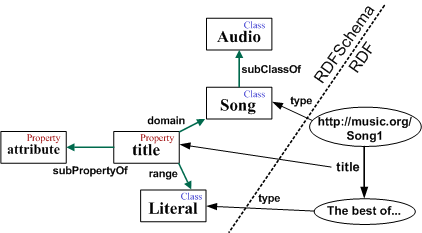
\includegraphics[height=2.5in]{images/RDFSchema.png}
	\caption{RDF Schema sample}
\label{fig:images_rdfs_sample}
\end{figure}

RDFS is described in RDF style using: \\
- core classes like: \\
  - `rdfs:Resource' (all objects/resources) \\
  - `rdfs:Class' (all classes) \\
  - `rdfs:Literal' (all literals) \\
  - `rdfs:Property' (all properties) \\
  - `rdfs:Statement' (all reified statements) \\
- core properties like: \\
  - `rdfs:type' (specify kind of class) \\
  - `rdfs:subClassOf' (specify inheritance between classes) \\
  - `rdfs:subPropertyOf' (specify inheritance between properties) \\
  - `rdfs:domain' (specify domain restrictions) \\
  - `rdfs:range' (specify range restrictions) \\
- container classes like: \\
  - `rdf:Bag'  (unordered list of entitites) \\
  - `rdf:Seq'  (ordered list of entities) \\
  - `rdf:Alt'  (list of alternatives/choices) \\
  - `rdf:Container' (superclass for all containers) \\
- utility classes like: \\
  - `rdfs:seeAlso', `rdfs:isDefinedBy' (links and references to other entities) \\
  - `rdfs:Comment' (comments and notes of entities) \\
  - `rdfs:Label' (human-friendly name of entities) \\
\\

Missing features in RDFS: \ldots  \\
\\
Complex Ontologies in Web Ontology Language (OWL): \\
\ldots \\
\\

% section semantic_ontologies (end)

\subsection{Query Language}
\label{sec:semantic_querylang}

SPARQL requires a \textbf{triple store} - a database containing RDF documents \\
is also referred to as a \textit{Graph Store} \\
data is inserted via Bulk load operation or via SPARQL update statements \\
SPARQL consist of SPARQL Queries that are send over the SPARQL protocol \\
Clients sends the queries to an HTTP endpoint \\
Stores on the public Web incl. dbpedia.org, ckan.org, wikidata.org \\
SPARQL also works with RDFS \\
SPARQL has similarities to SQL:
- each element in a triple might be replaced with a variable like `?varName' like so: \\
\texttt{sample.sparql:}
\begin{lstlisting}[basicstyle=\ttfamily,numbers=left,numberstyle=\footnotesize\ttfamily,backgroundcolor=\color{sourcegray}]
  PREFIX ns1:<URI>
  PREFIX ns2:<URI>
  PREFIX ns3:<URI>

  SELECT ?varName
  WHERE {
      ns1:subject ns2:predicate ?varName
  }
\end{lstlisting}
- in the WHERE clause it hosts the graph pattern to match (could be cascaded to go down subgraphs) \\
- variables can occur at any place in the graph pattern (?subj ?pred ?obj) as select with query everything \\
\\
LIMIT \textless n\textgreater option at the end for limiting the result set \\
FILTER (?varName \textless condition\textgreater ) in graph pattern can restrict results to match some
literal values and supports: \\
- numbers, dates: \textless, \textgreater, = \\
- strings: =, regex() \\
\\
\textbf{open world} assumption: resources on the Web are described in different schematas with various properties
using different vocabularies \\
- UNION option in graph pattern combines different matches \\
- OPTIONAL option in graph pattern only returns those entities if they are available (otherwise empty) \\
\\
ASK query checks for the existence of a given graph pattern \\
CONSTRUCT can be used to retrieve a subgraph from a larger graph, can also be used to translate between different schemas \\
\texttt{sample2.sparql:}
\begin{lstlisting}[basicstyle=\ttfamily,numbers=left,numberstyle=\footnotesize\ttfamily,backgroundcolor=\color{sourcegray}]
  PREFIX ns1:<URI>
  PREFIX ns2:<URI>
  PREFIX ns3:<URI>

  CONSTRUCT {
      ?varA ns2:predicate ?varB .
      ?varA ns3:predicate ?literalA .
  }
  WHERE {
      ?varA ns1:predicate ?varB
  }
  FILTER ( ?varB > x )
\end{lstlisting}

- SPARQL can be used to harmonize graphs from different sources \\
- is also used for basic reasoning ala ``if found this, assume that'' \\
- can ease hierarchical queries with * or + on the predicate (SPARQL 1.1) \\
- can help resolving issues with different entities referring to the same object (MKP pg. 95)\\
- Federated Queries can be used to combine information from distinct sources via SPARQL (MKP pg. 110-112)\\
\\
- inferencing information from existing triples via SPIN (SPARQL Inferencing Notation) \\
- like in a taxonomy items can be categorized in an hierarchy (MKP pg. 114) \\
- inference patterns are used in Semantic Web applications (MKP pg. 115) \\
   * subClassOf - type propagation rule \\
- inferencing could be done at query time or persistently (MKP pg. 120/121) \\
- inferences can also be helpful when combining information from unknown sources \\
- inferencing happens on various levels (RDFS, RDFS+, OWL) with an increased set of complex inferencing rules (MKP pg. 122/123)
\\
% section semantic_querylang (end)

\subsection{Agents and Rules}
\label{sec:semantic_logic_rules}


% section semantic_logic_rules (end)

% section semantic_web (end)
